\subsection{Game Interface}

\subsubsection{Main Interface}

The main interface consists of several parts, a chess board, the area of players' hands, the display of the scoring combinations, the functional explanation of all action tokens, the demonstration of two team score points, and the label of the current player. 

\begin{enumerate}
	
	\item\textbf{Menu bar}\\
    In the main interface, the menu bar is apart into two separate sections. The first bar is called "setting", which obtains four menu items for the fundamental setting of the game, as Figure \ref{fig:settingMenu} below. 
	\begin{itemize}
		\item{Setting} \\ 
		\begin{itemize}
			\item {New Game} \\ 
		    The aims of the Menu item of New Game are used for creating a new game. 
			
			\item {Save} \\
			The aim of Menu item Save is used to save an incomplete game. The saving file is using GSON to translate the whole game system, including every player's state, the current board, the remained action tokens, and the current player.  
			
			\item {Load} \\
			The aim of Menu item Load is used to load a given game. A given file is provided with JSON and it can be analysed by using GSON to the whole game system, including every player's state, the current board, the remained action tokens, and the current player.  
			
			\item {Close} \\ 
			The function of Menu item Close is closing the game. 
			
		\end{itemize}
		
		
		\begin{figure}[h]
			\centering
			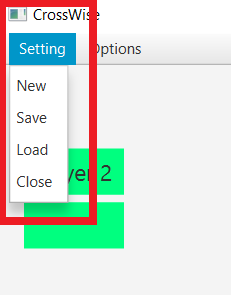
\includegraphics[width=0.3\textwidth]{image/settingMenu}
			\caption{The setting menu item}
			\label{fig:settingMenu}
		\end{figure}
		
		\newpage
		\item{Options} \\ 
		The options menu Figure \ref{fig:optionsMenu}  and explanation are shown below:
		\begin{itemize}
			\item {Duration} \\ 
			The menu item Duration contains three subdivisions, short, medium, and long, which are for dominating the duration of highlighting a cell on the chess board. 
			
			\item {Row/Column Score Display} \\
	    	The menu item Display Row/Column Score controls the visibility of seeing the score of each row and column. The default setting is invisible for all rows and columns.  
			
			\item {Current Team Points} \\
			The menu item Current Points controls the visibility of seeing the current total points of two teams. The default setting is invisible for the current team point.
			
			\item {Computer Hands} \\
			The menu item Computer Hands is utilized to manipulate the exhibition of the computer hands token. As there are bots participating in a game, the menu item could be executed for deciding whether their hands token should be visible or not. 
			
			\item {Stop AI playing} \\ 
	    	The menu item Stop AI Playing can be used to interrupt and cease the game when all players are a bot. The default setting is that this menu item is able implemented when all players are bots. 
			
		\end{itemize}
		
		\begin{figure}[h]
			\centering
			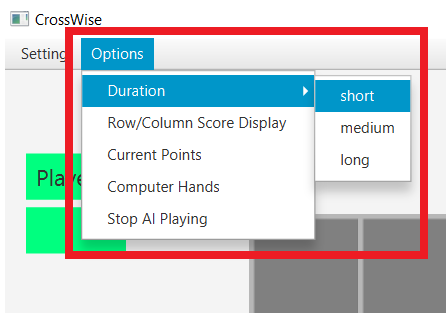
\includegraphics[width=0.5\textwidth]{image/OptionsMenu}
			\caption{The option menu}
			\label{fig:optionsMenu}
		\end{figure}
		
		
	\end{itemize}
	\newpage
\item\textbf{Chess board}\\
The chessboard is made of a 7x7-table, which is used for placing symbol tokens and displaying the score points of each line. Among, the 6x6-table where symbol tokens can be settled in each cell, is entirely occupied with a symbol token called None. Additionally, the endmost row and column remain empty in order to show the scoring point of each line. The graphic is shown below Figure \ref{fig:chessboard} .

\begin{figure}[h]
	\centering
	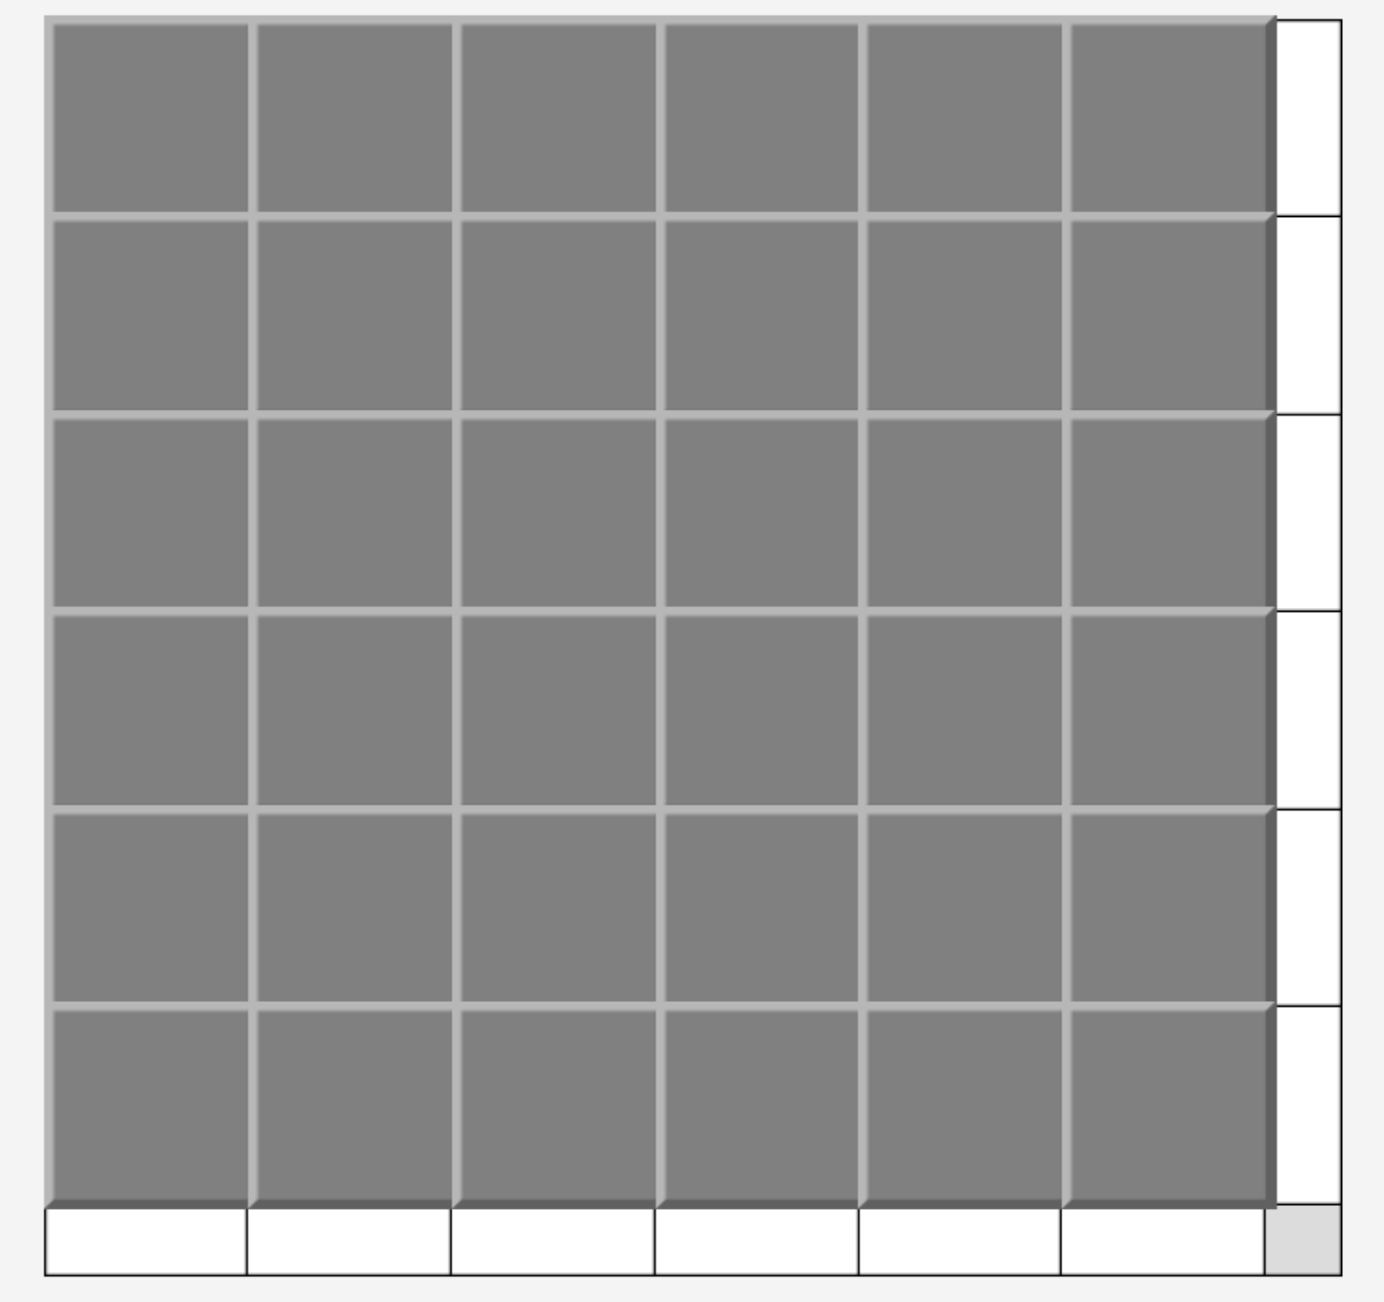
\includegraphics[width=0.6\textwidth]{image/chess board}
	\caption{The chess board}
	\label{fig:chessboard}
\end{figure}

\newpage
\item\textbf{Players' hands}\\ 
As shown in the Figure \ref{fig:playerhand} below, there are four red marking areas that surround the chess board, those areas are the players' hand tokens. 
If there are only two players involved in the game, then the exclusive area which is for player 1 and player 2 is visible..  

\begin{figure}[h]
	\centering
	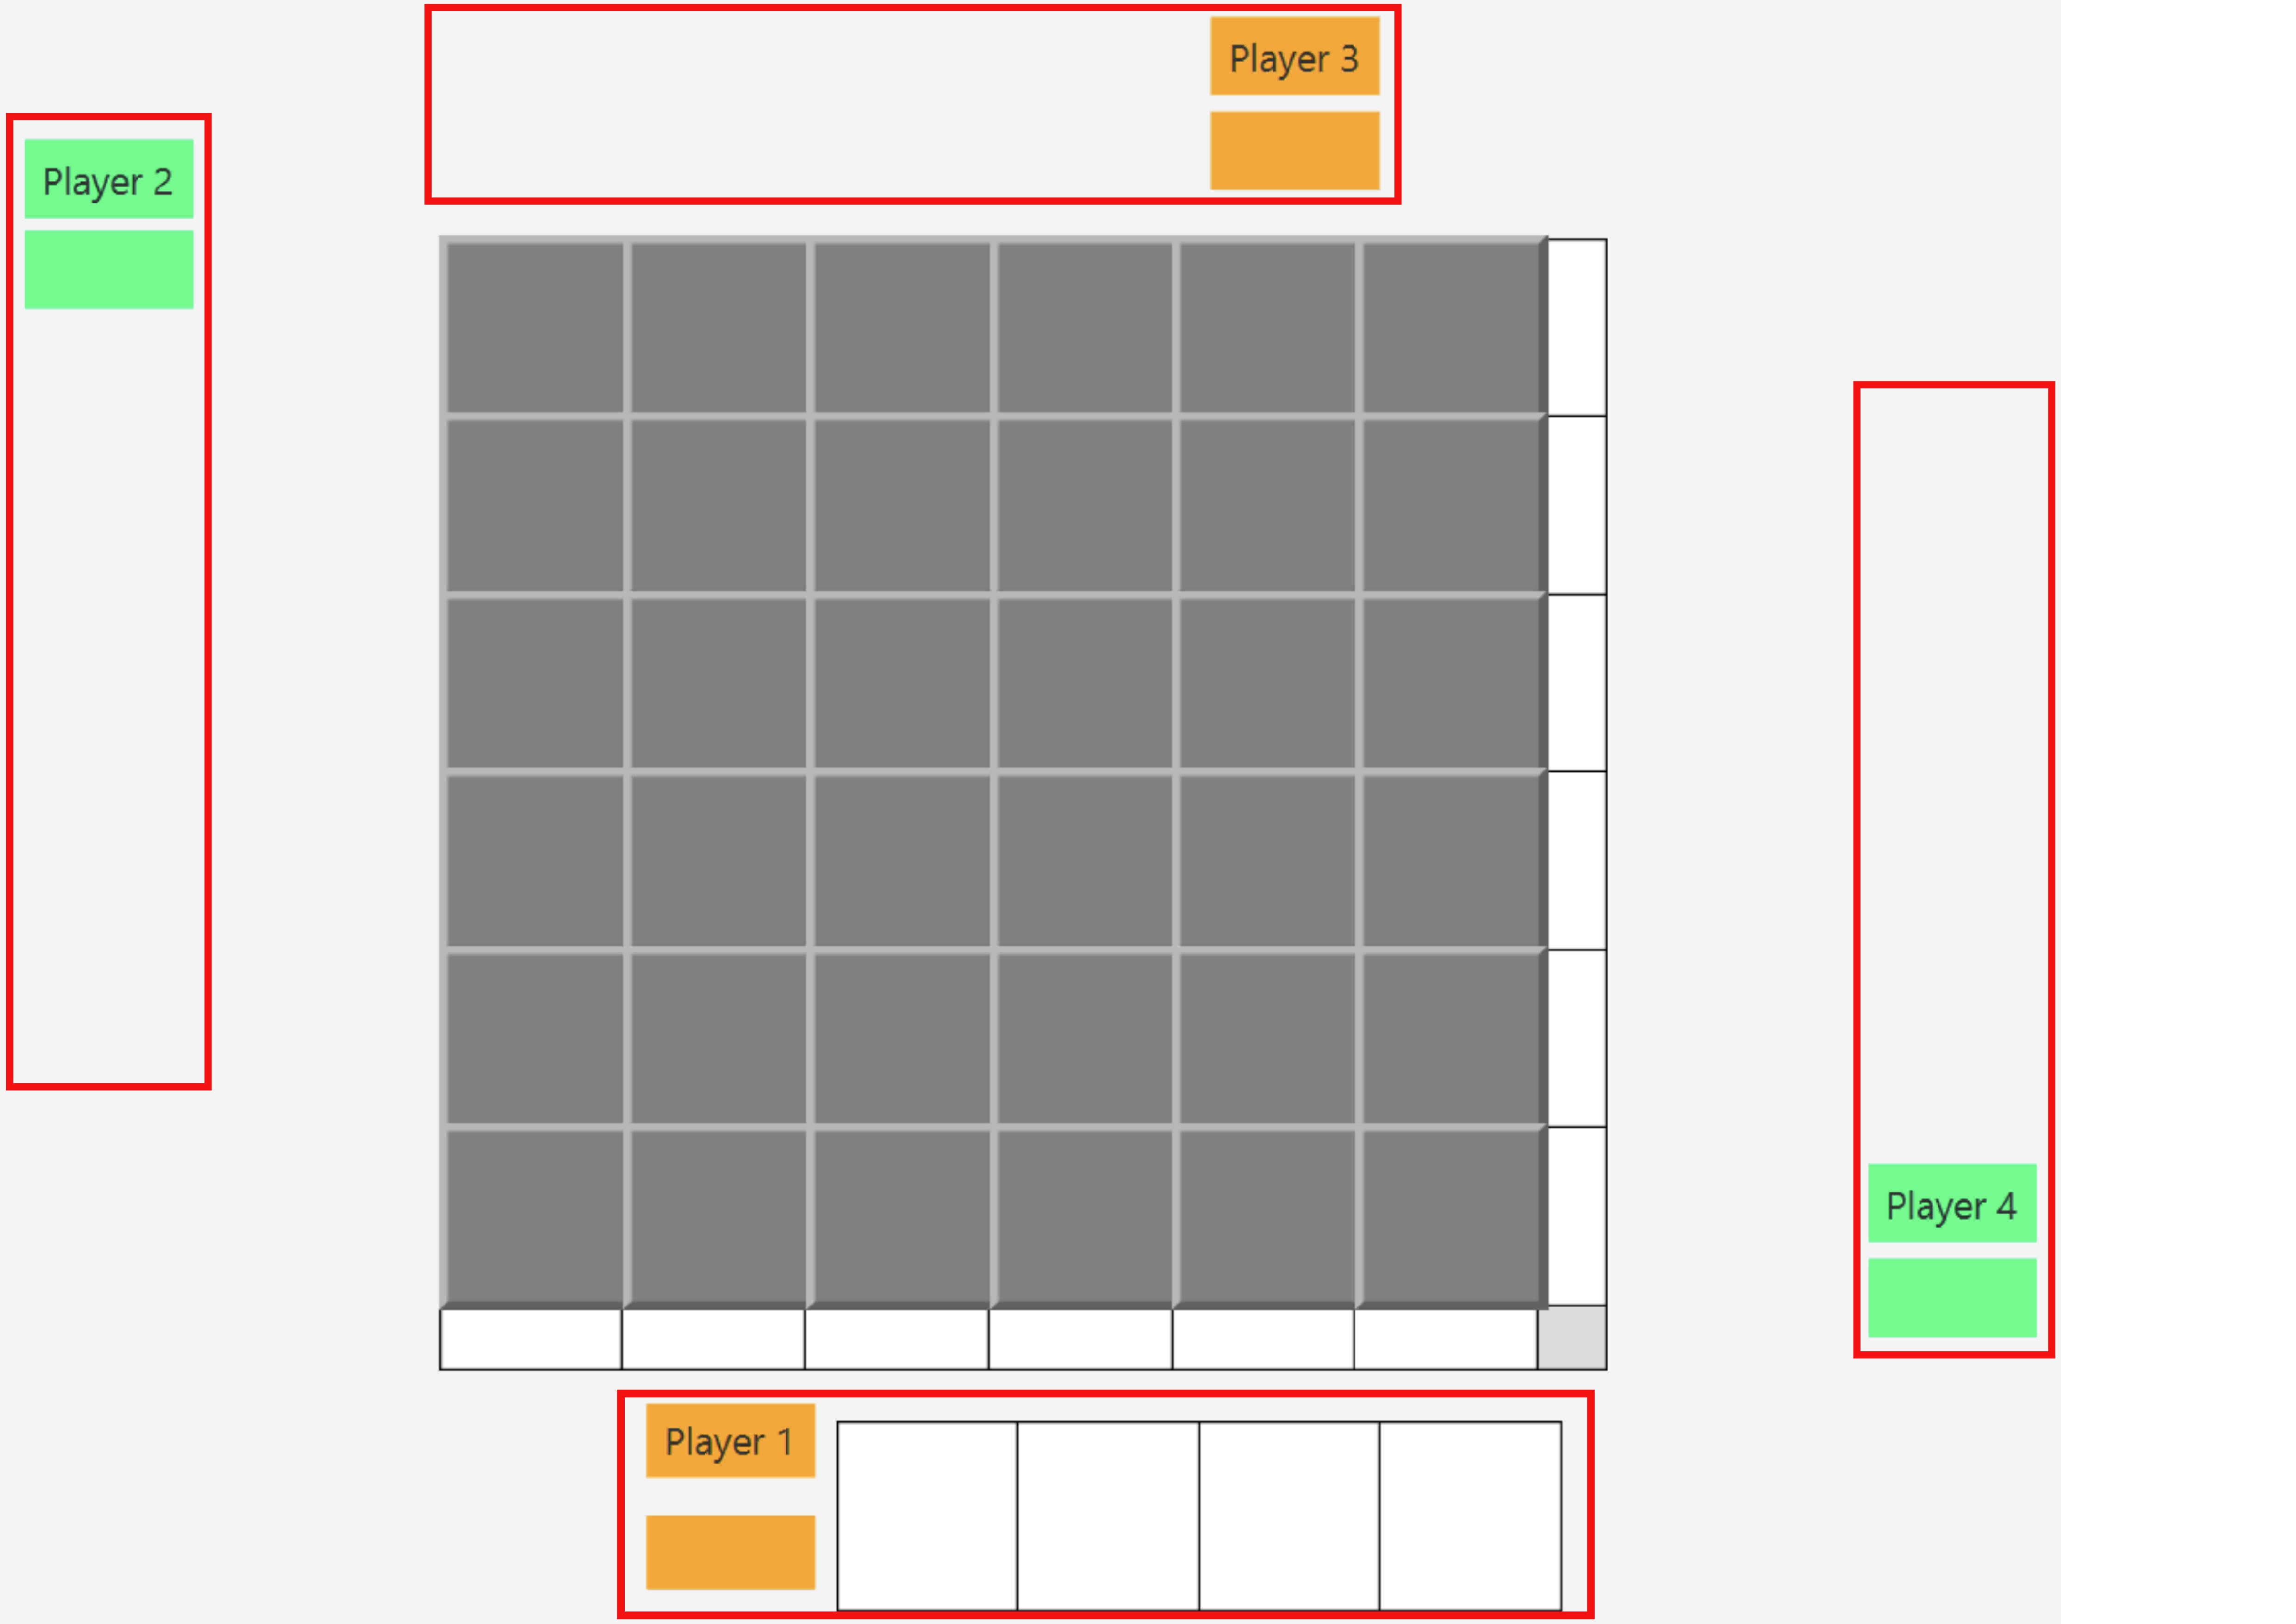
\includegraphics[width=0.8\textwidth]{image/players' hands }
	\caption{Players' hands}
	\label{fig:playerhand}
\end{figure}


\item\textbf{The combination of the scoring points }\\
On the right side of the main interface, a zone is for displaying all attainable combinations of every score. While the player is in the progress of the game, it is possibly forgotten how is the point being calculated. Hence, this region can remind players of the scoring logic. The demonstration is shown below in Figure \ref{fig:scoring points}.

\begin{figure}[h]
	\centering
	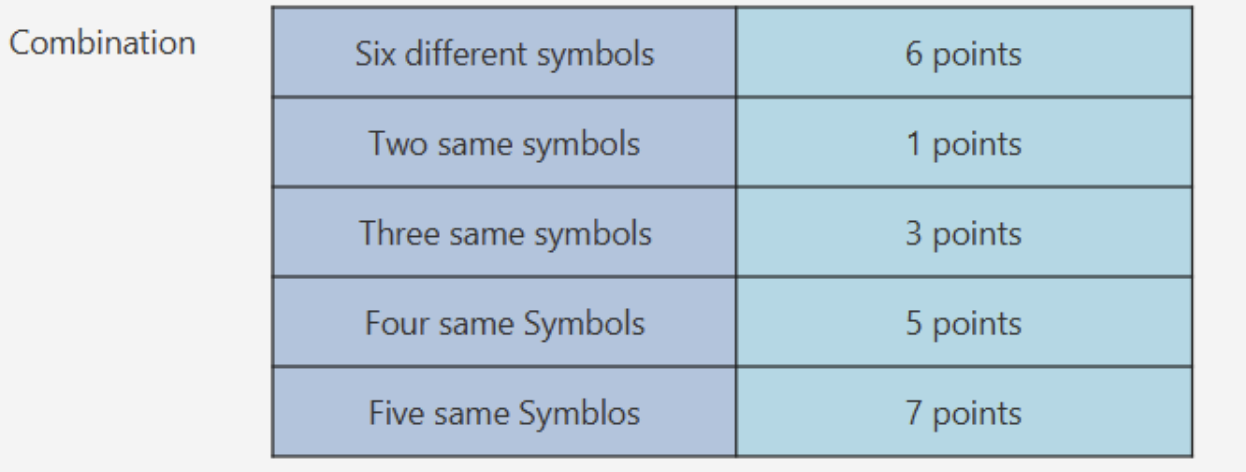
\includegraphics[width=0.8\textwidth]{image/scoring points}
	\caption{The combinations of scoring points}
	\label{fig:scoring points}
\end{figure}

\newpage

\item\textbf{The demonstration of two team score}\\
Undeniably, if the player can regularly inspect their current achievement, the experience of the game, and the convenience of the exploring game are increased undoubtedly. Therefore, possessing an area that demonstrates the achievement of two teams is a necessary arrangement. The demonstration is shown below in Figure \ref{fig:teamscore}.

\begin{figure}[h]
	\centering
	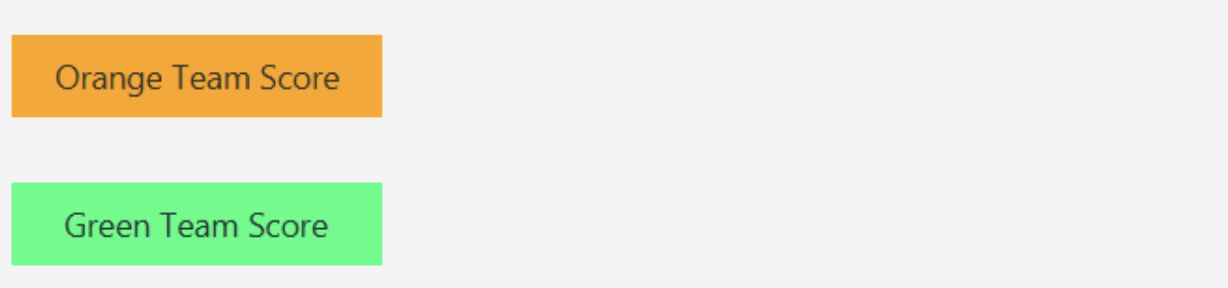
\includegraphics[width=0.8\textwidth]{image/two teams score}
	\caption{The display of team scores}
	\label{fig:teamscore}
\end{figure}

\item\textbf{The label of the current player}\\
As with the display of two team scores, labelling a current player is also an excellent option to enable participants to realize who turns. Meanwhile, the background colour of this label can be varied as the team belongs to the current player. The label is shown below in Figure \ref{fig:currentPlayer}.

\begin{figure}[h]
	\centering
	
\includegraphics[width=0.8\textwidth]{image/current Player}
	\caption{The label of current players}
	\label{fig:currentPlayer}
\end{figure}

\item\textbf{The explanation of all action tokens}\\
As with the same purpose of exhibiting combinations of the scoring points, having a description for action tokens provide considerable benefits for the game. Players can be reminded of the function of those four action tokens. 

Moreover, on the right side of the figure \ref{fig:the demonstration of action token} shown below, a list of the remaining number of action tokens is exhibited. Once one of these action tokens has been utilized, the list of the remaining number of action tokens will be updated automatically.  

\begin{figure}[h]
	\centering
	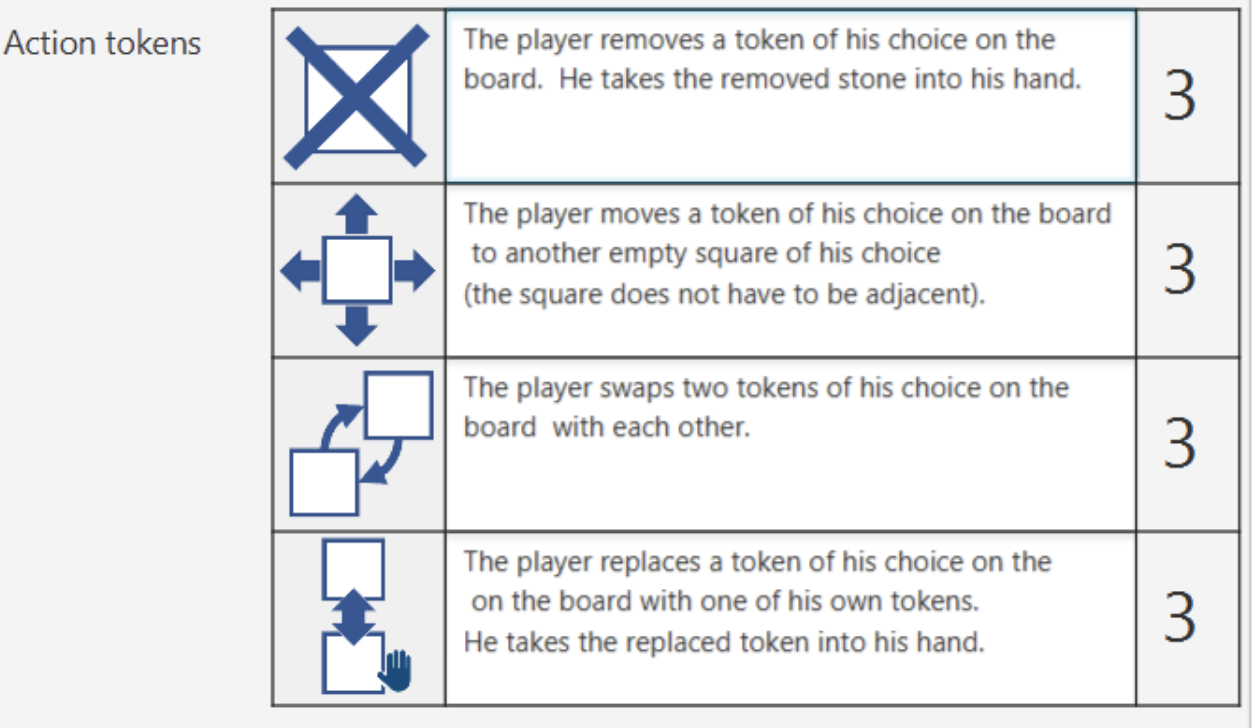
\includegraphics[width=0.6\textwidth]{image/the demonstration of Action token}
	\caption{The demonstration of action tokens}
	\label{fig:the demonstration of action token}
\end{figure}

\end{enumerate}

\newpage
\subsubsection{Secondary Interface}

\begin{enumerate}
	\item\textbf{Menu bar}\\
	The red marked area of the Figure \ref{fig:secondWindowMenu} represent the options menu items for deciding participants' number in a game. The default setting for initiating a game is four players.
	
	\begin{figure}[h]
		\centering
		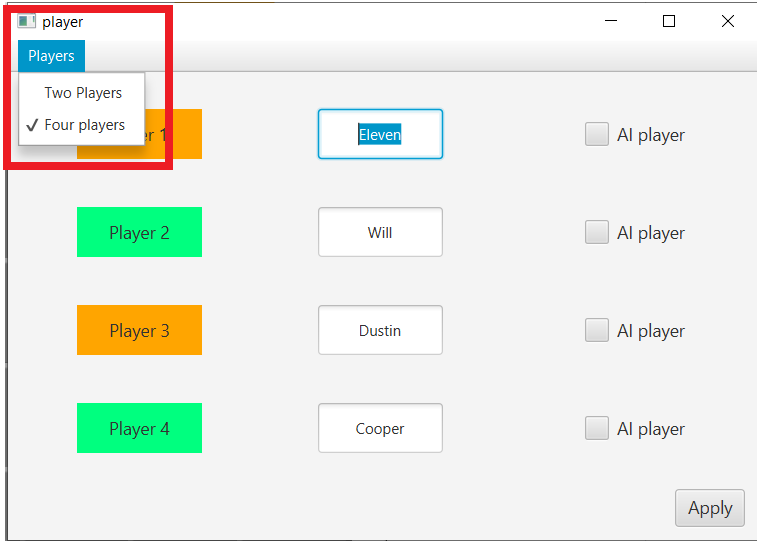
\includegraphics[width=0.6\textwidth]{image/secondWindowMenu}
		\caption{The menu bar in the second window}
		\label{fig:secondWindowMenu}
	\end{figure}
	
	
	
	\item\textbf{The second window}\\
	The Figure \ref{fig:playerScene} below represent an interface for initializing the state of players, involved in establishing player amounts, inputting players' name, and determining the state of the player in human or bot. As you can see the top-left corner has a menu item that can set up the number of players in a game. And in the middle of this scene which is circled as blue, there are four labels that can be entered players' names. At last, the right side of the scene which is marked as red provides four check boxes that enable the user to determine which players are manipulated by AI or humans.  
	
	\begin{figure}[h]
		\centering
		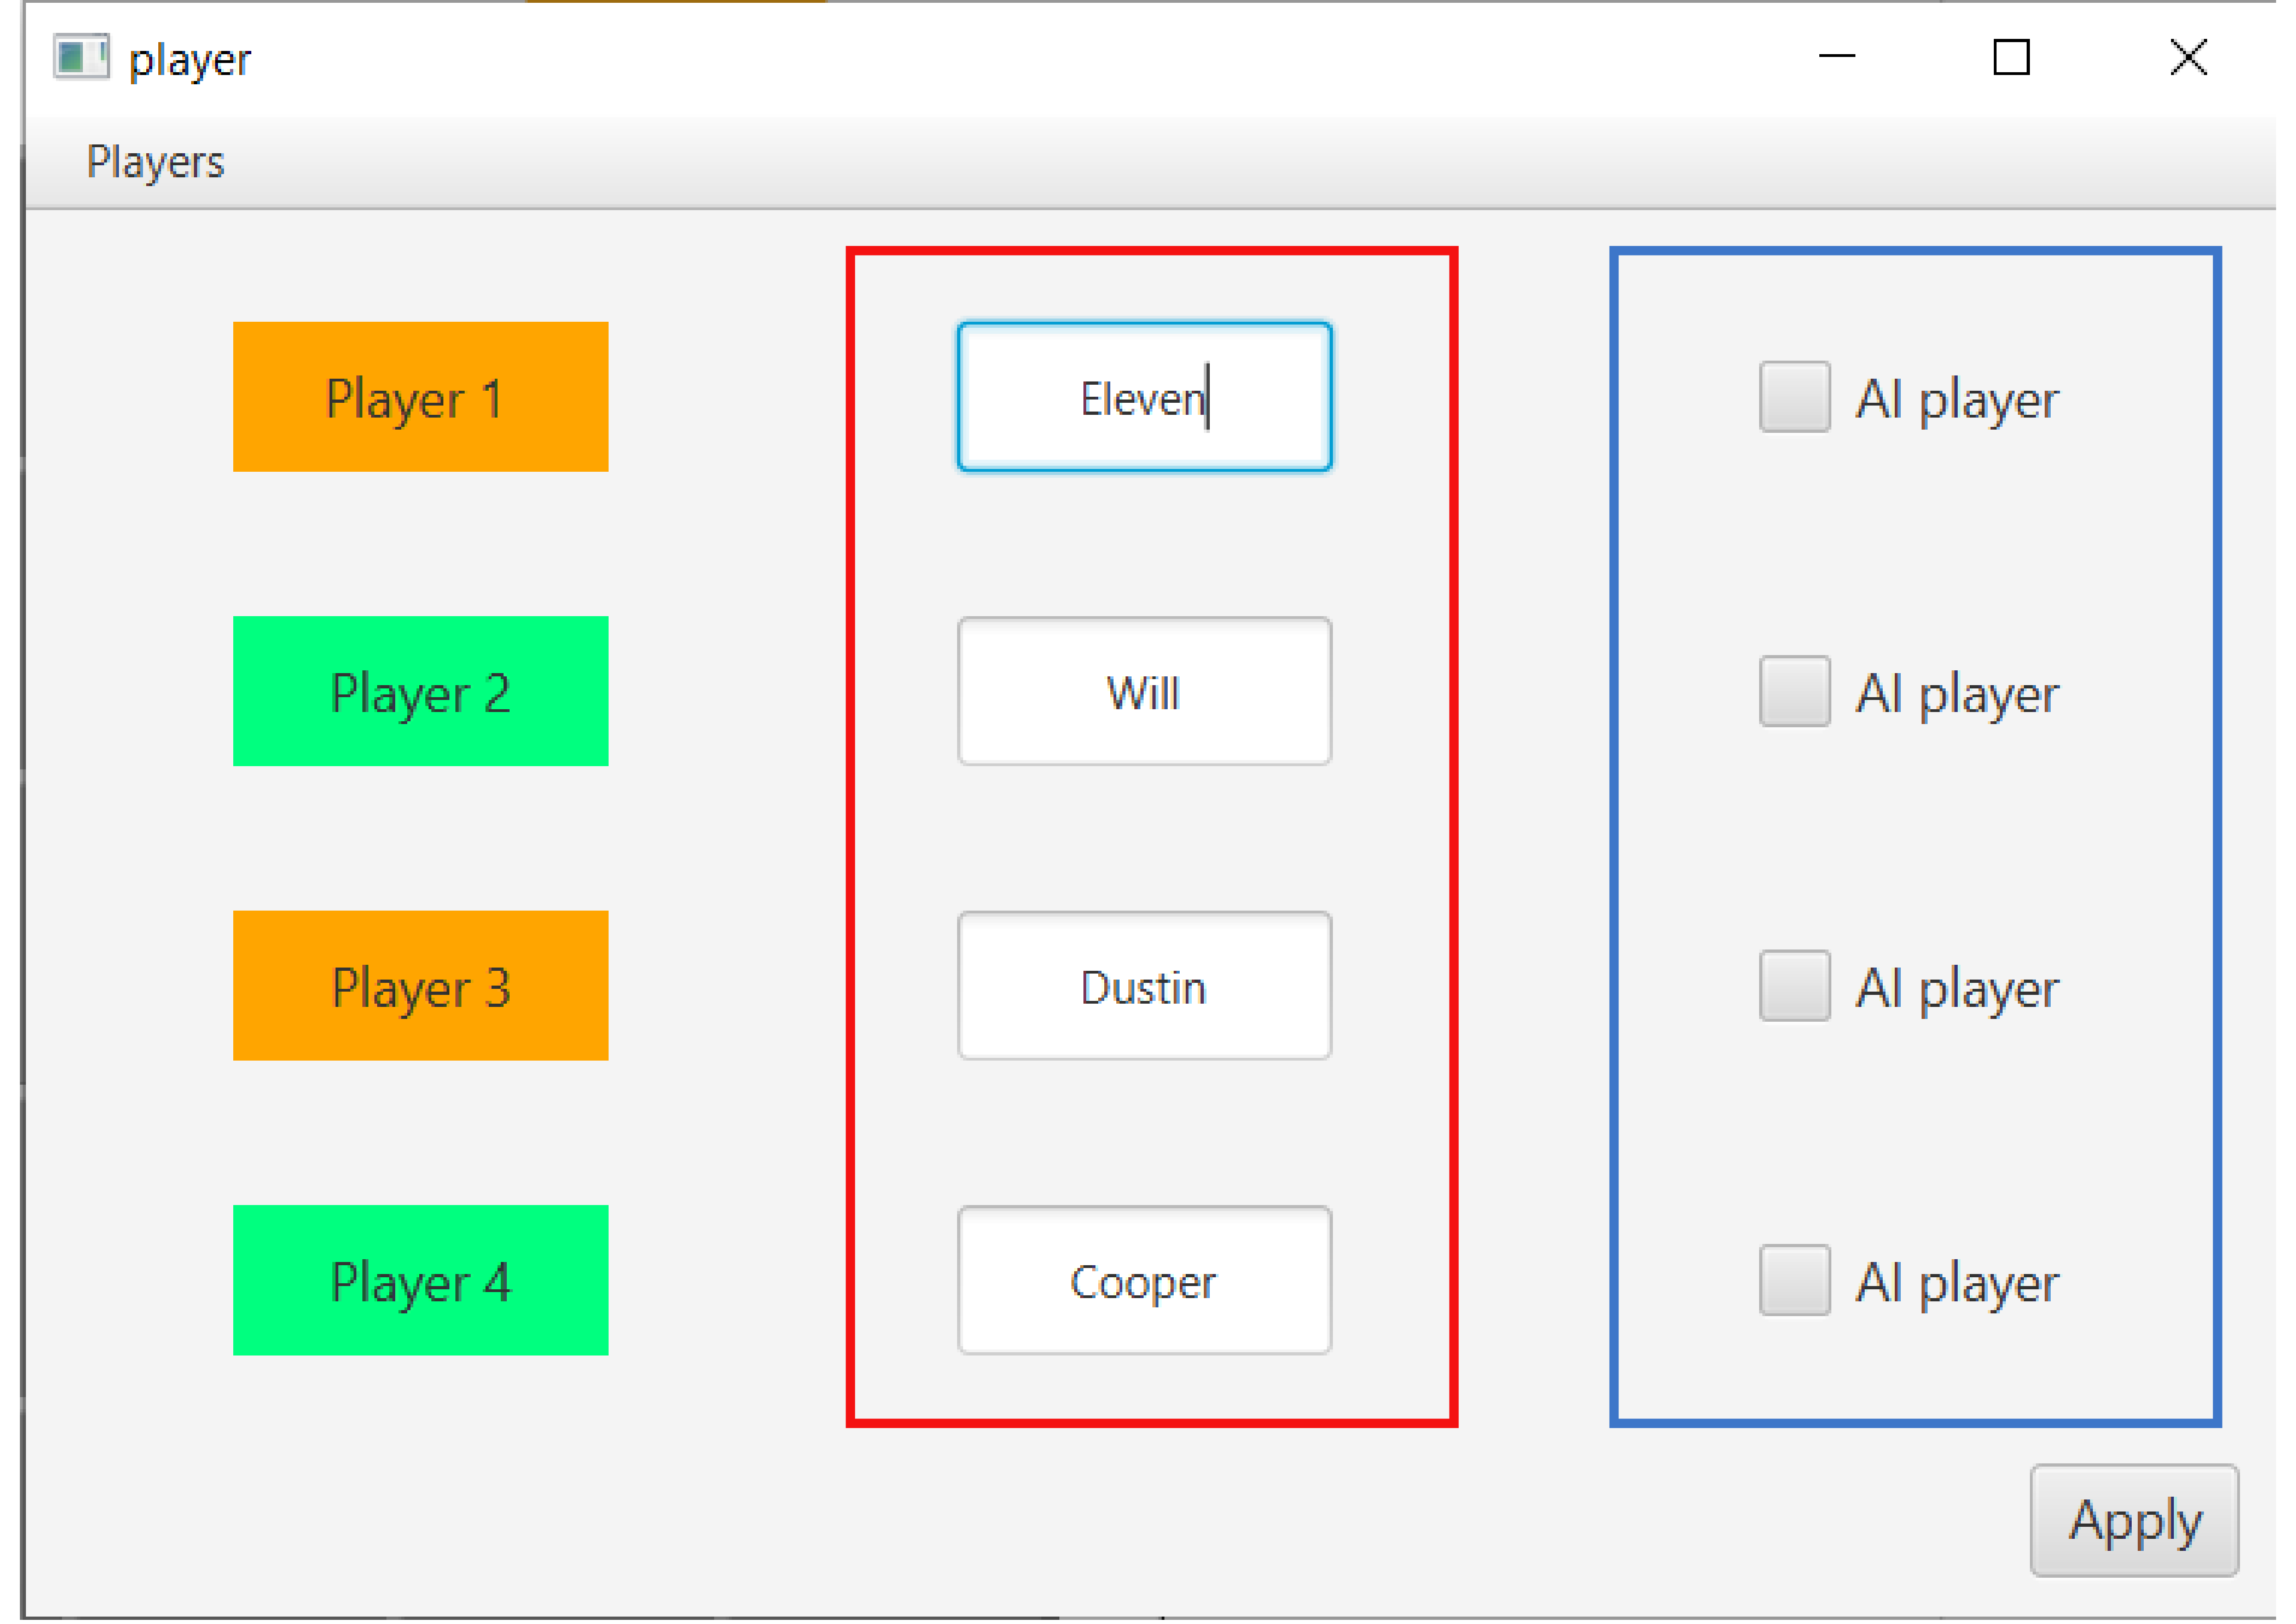
\includegraphics[width=0.6\textwidth]{image/Player scene}
		\caption{The second interface - player scene}
		\label{fig:playerScene}
	\end{figure}
\end{enumerate}

\newpage